\chapter{Measurement and Evaluation}
\sout{Here presents the measurement we used to analysis the change / optimization, as well as corresponding results (and graphs / figures).
If we can finish more assumptions (\eg investigate clustering), the following part goes in different subsections.}

Researchers always want to get results faster, so they will prefer frameworks that could use less time to finish calculation. We will now do measurement and perform evaluation of the results to show the performance of our extension to dispel4py.

We will make measurements on each of the extensions we've created. Each of them goes into a subsection below, and contains the main property of the measurement.
\section{Incremental deployment}
\sout{How to measure, what to measure  (mainly those described in the measurement plan).
Results (figures) and analysis.}

\section{Dynamic expansion}
Dynamic expansion is the new property we have added to dispel4py system. It creates a new semantics to workflow design so that workflows can grow / expand according to needs. We use the sieve of Eratosthenes to demonstrate the potential usage of this new semantics, and make comparisons between the approaches we need to construct such a workflow graph in both the old system and our new system, and the performance of the old system (constructed in the old way) and the new system (constructed in the new way).

The original structure of the sieve of Eratosthenes is fairly simple: list all digits (up to a number), and go from the first one (2) till the last one (except for those crossed) to cross all digits that are multiple of the current digit. To write it into code, it will look like this:

PSEUDOCODE HERE

To write a workflow which utilizes the sieve of Eratosthenes without \emph{dynamic expansion},  researchers need to first write down the range of numbers (which is always needed), and then estimate (or calculate) the number of primes inside this range. This is a chicken-and-egg problem: we need to execute the whole workflow to know \textbf{what} primes are there inside this range and then can know the \textbf{number} of primes inside this range; but we also need the \textbf{number} of primes to design the workflow (which is prior to the execution of this workflow). Therefore, there are two ways to ``solve'' this problem:
\begin{enumerate}
	\item Run the calculation somewhere else and use that result.
	\item Estimate a bigger number and hope the actual number of primes won't exceed it.
\end{enumerate}

Apparently these two ways are not neat, and there isn't a neat way to solve this problem in the old semantics. However, in our new system with \emph{dynamic expansion}, this problem automatically goes away: researchers simply need to define when to dynamically expand this node as a part of the construction of the Sieve PE, and add \textbf{one} of it into the workflow. Figure \ref{fig:comp_old_new_sieve} shows the structure of workflow design in the old system and the new system.

\begin{figure}[h]
\caption{
TWO FIGURES HERE:
the first one shows the structure of the old semantics (with one IntegerProducer and many Sieves);
	the second one shows the structure of the new semantics (with only two nodes: IntegerProducer and Sieve)
}
	\label{fig:comp_old_new_sieve}
\end{figure}

The results are shown in figure \ref{fig:sieve_all}

\begin{figure}[h]
\centering
    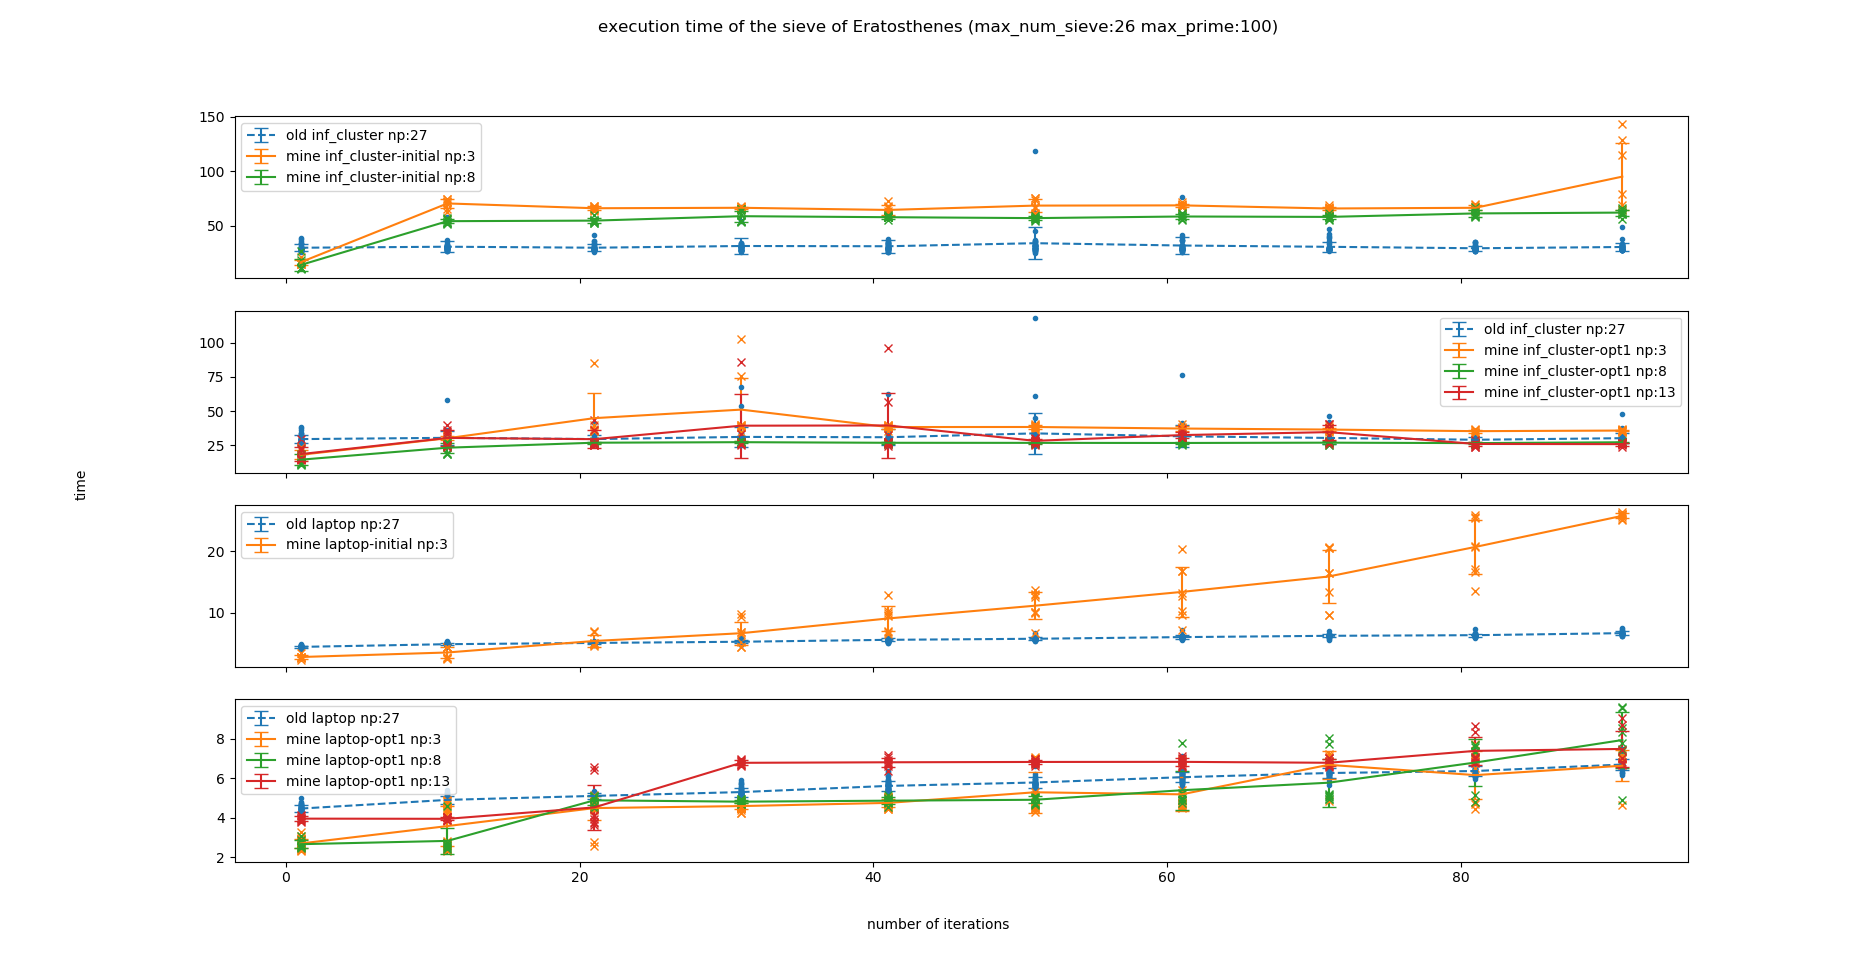
\includegraphics[width=1\textwidth]{figures/sieve_all_100}
    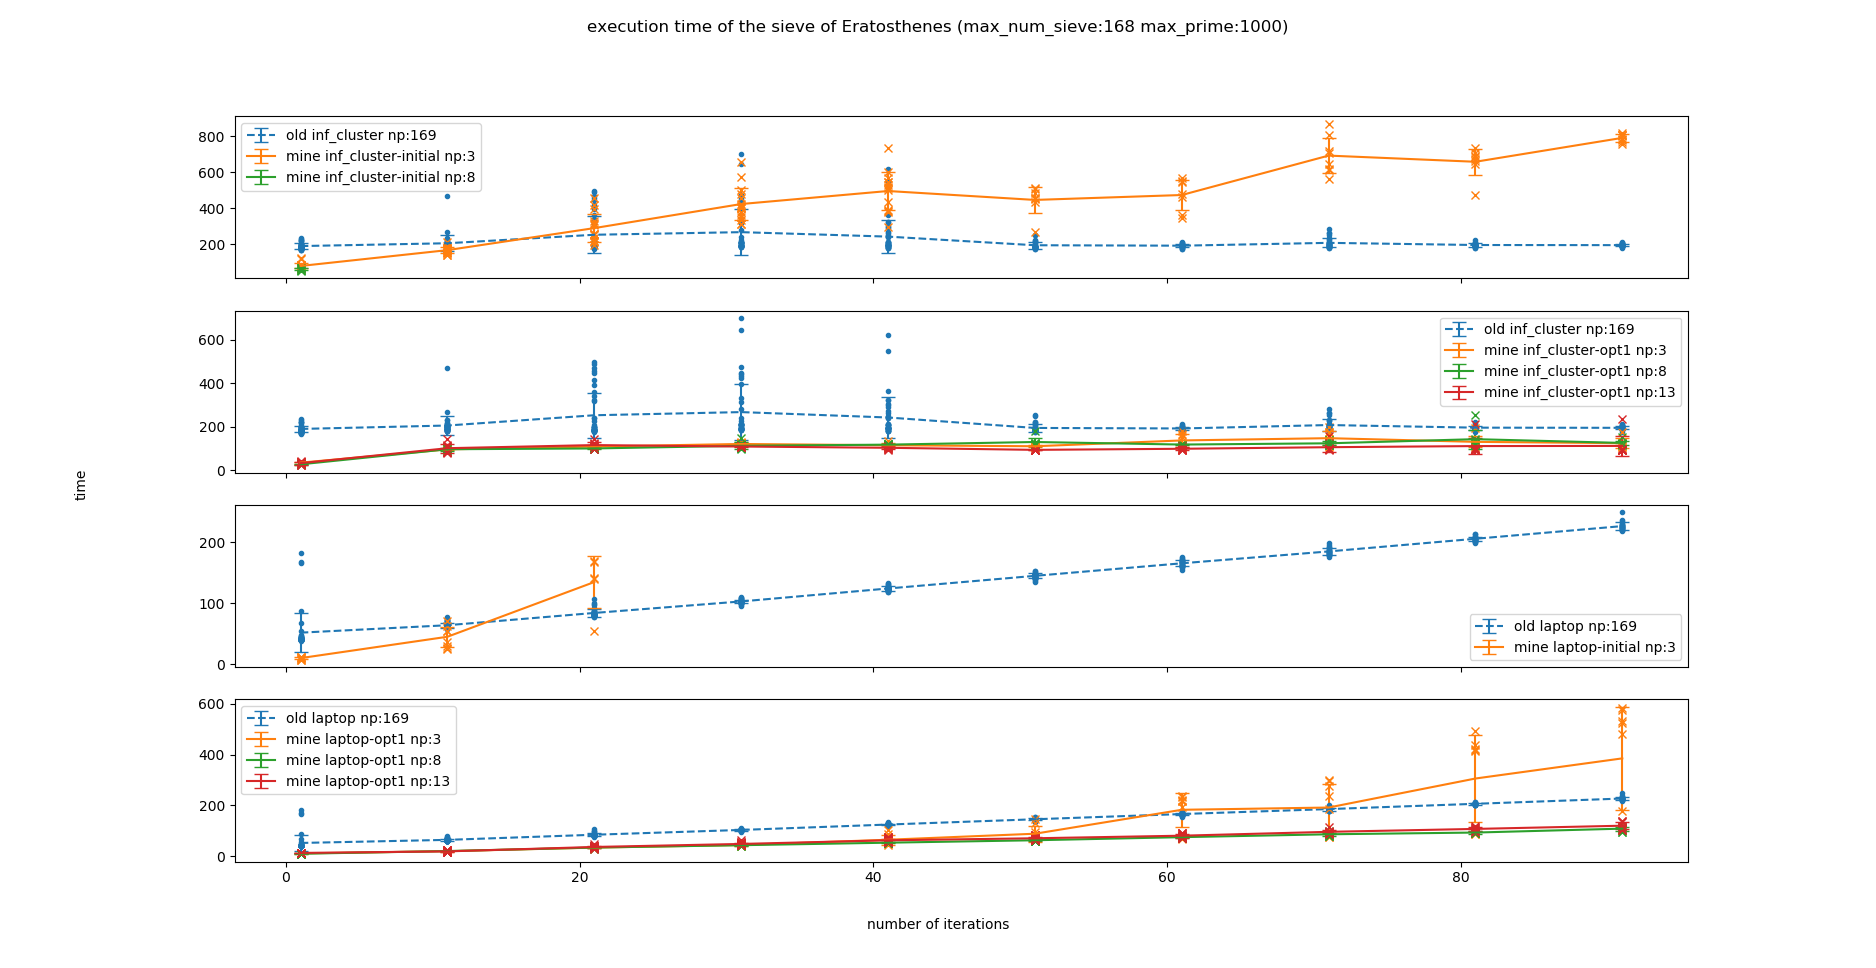
\includegraphics[width=1\textwidth]{figures/sieve_all_1000}
\caption{Execution time of the sieve of Eratothesnes on both the old semantics and our new semantics.
The second column of the legend indicates the platform and the version (separated by a dash), and the third column of the legend is one of the parameters controlling the number of nodes spawned at the beginning}
\label{fig:sieve_all}
\end{figure}

\begin{figure}[h]
\centering
    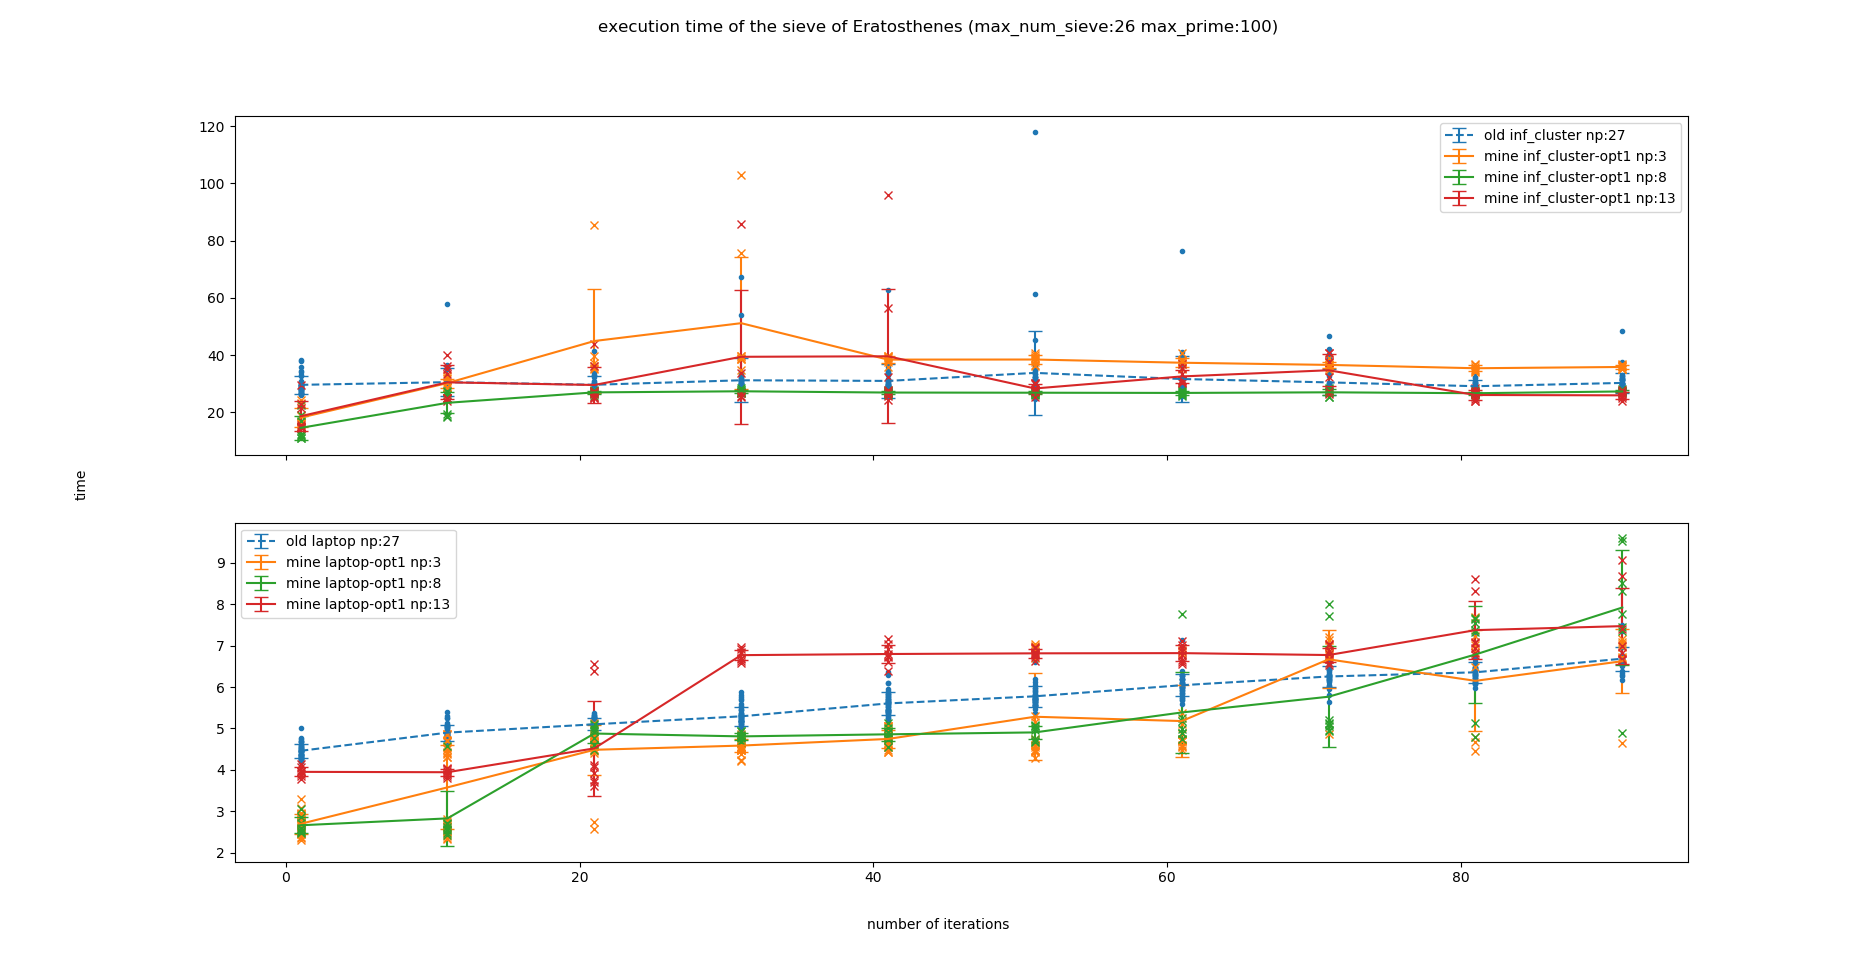
\includegraphics[width=1\textwidth]{figures/sieve_opt1_100}
    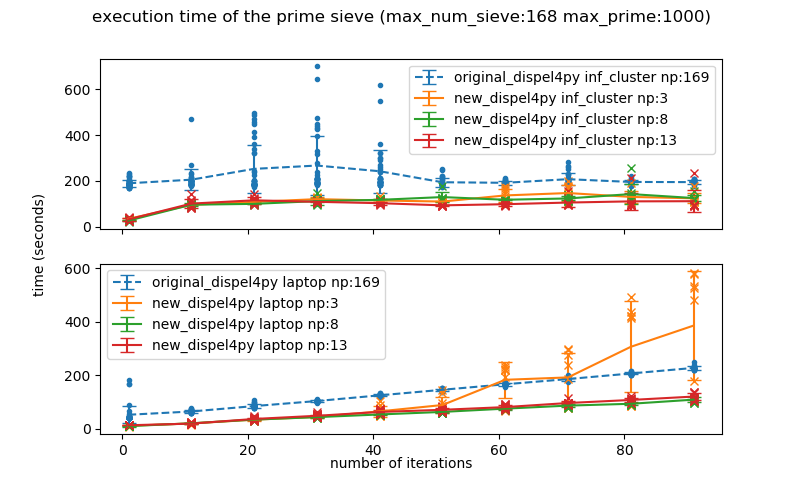
\includegraphics[width=1\textwidth]{figures/sieve_opt1_1000}
\caption{Execution time of the sieve of Eratothesnes on both the old semantics and our new semantics (only the optimized version)}
\label{fig:sieve_opt1}
\end{figure}
